\documentclass{article}
\usepackage{tikz}
\usepackage{pgf}
\usepackage[utf8]{inputenc}
\usepackage{pgfplots}
\usepackage{pgfplots}
\usepgfplotslibrary{patchplots,colormaps}
\pgfplotsset{compat=1.9}
\usepgfplotslibrary{groupplots,dateplot}
\usetikzlibrary{patterns,shapes.arrows}
\usepackage{amsmath}
\usepackage{amssymb}
\usepackage{xcolor}
\usepackage{tikz}
\usepackage{pgfplots}
\usetikzlibrary{matrix,positioning}
\usetikzlibrary{automata,positioning,arrows.meta,math,external}
\usetikzlibrary{decorations.pathreplacing}
\usetikzlibrary{shapes,shapes.geometric, snakes}
\usetikzlibrary{arrows, chains, fit, quotes}

\begin{document}

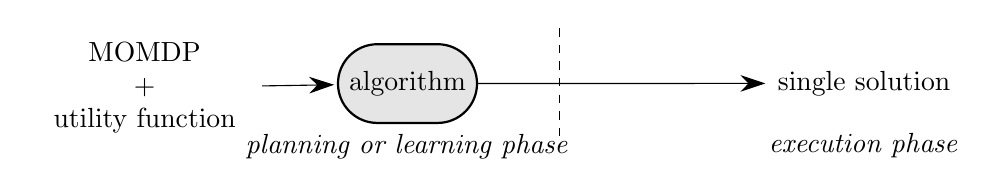
\begin{tikzpicture}[>={Stealth[width=6pt,length=9pt]}, skip/.style={draw=none}, shorten >=1pt, accepting/.style={inner sep=1pt}, auto]
\draw (-20.0pt,20.0pt) node[below](0) {\begin{tabular}{c} MOMDP \\ + \\ utility function \end{tabular}} ;
\draw (75.0pt, 0.0pt) node[rounded rectangle, thick, fill=gray!20, minimum height=1cm,minimum width=2cm, draw, label=below:$\text{\emph{planning or learning phase}}$](1){$\text{algorithm}$};
\draw (240.0pt,14.5pt) node[below, minimum height=1cm,minimum width=2cm, label=below:$\text{\emph{execution phase}}$](2){$\text{single solution}$} ;
\draw [dashed] (130.0pt,20pt) -- (130.0pt,-20.0pt);
\path[->] (0) edge node{} (1);
\path[->] (1) edge node{} (2);
\end{tikzpicture}

\end{document}